\section{Fabrikmethode}

\begin{figure}[h]
\centering
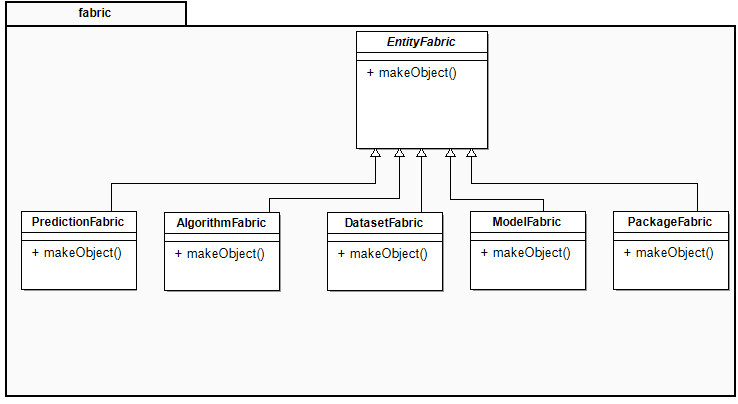
\includegraphics[width=0.6\linewidth]{Grafik/Klassendiagramme/fabrik.png}
\caption{Fabrikmethode zur Erzeugung der MVC Instanzen}
\end{figure}


Die Erstellung der bereits eben erwähnten Model-View-Controller-Struktur der Entitys wird über eine Abstract Factory geregelt. Dieses Pattern sorgt dafür, dass immer der richtige Controller zusammen mit der richtigen View und dem entsprechenden Model erstellt wird.

%@Markus: Im Zweifelsfall hau hier einfach nur die Grafik von der Fabrik rein
%... falls mir noch irgend ein halbwegs sinnvoller Text dazu einfällt ergänz ich den 